\section{Clasificaci\'on Supervisada: An\'alisis Discriminante}

\begin{itemize}
    \item Tablas de datos con $n$ individuos, $p$ variables y una variable categórica $G$ con $q$ niveles.
    
    \begin{center}
        \begin{tabular}{|cccc|c|}
            \hline
               $X_1$ &    $X_2$ & $\cdots$ &    $X_p$ &      $G$ \\
            \hline
            $x_{11}$ & $x_{12}$ & $\cdots$ & $x_{1p}$ &    $g_1$ \\
            $x_{21}$ & $x_{22}$ & $\cdots$ & $x_{2p}$ &    $g_2$ \\
            $\vdots$ & $\vdots$ & $\ddots$ & $\vdots$ & $\vdots$ \\
            $x_{n1}$ & $x_{n2}$ & $\cdots$ & $x_{np}$ &    $g_n$ \\
            \hline
        \end{tabular}
    \end{center}

    \item El objetivo es determinar para un nuevo paciente $x_{(n+1)}$ con $X_1=x_{(n+1)1},\dots,X_p=x_{(n+1)p}$ su clasificación en $G$.
    \item \textbf{Muestra patrón:} Se llama muestra patrón (o \textit{train-data}) al conjunto de observaciones pareadas con su grupo. $\mathcal{Z}=\{x_i,g_i\}_{i=1}^n$
    \item \textbf{Regla de Bayes:} Asignaremos $x$ al grupo $K$ si
    \[
        \pi_Kf_K(x)=\max_{k=1,\dots,q}\pi_kf_k(x)
    \]
    \item Se utiliza la información disponible en $\mathcal{Z}$ para obtener $\hat{\pi}_k$ y $\hat{f}_k(x)$.
    \item \textbf{Normal multivariante:} $X=(X_1,\dots,X_p)'$ sigue una distribución normal $p$-variante $X\sim N_p(\mu,\Sigma)$ si admite densidad
    \[
        f(x;\mu,\Sigma)=\frac{1}{(2\pi)^{p/2}|\Sigma|^{1/2}}\text{exp}\left\{-\frac{1}{2}(x-\mu)'\Sigma^{-1}(x-\mu)\right\} \quad \forall x \in \mathbb{R}^p
    \]
    \item Elipsoides de equidensidad: $\{x:(x-\mu)'\Sigma^{-1}(x-mu)=\text{cte.}\}$
    \item \textbf{Distancia de Mahalanobis:} Mide la distancia de $x$ al centro de la distribución $\mu$ teniendo en cuenta la ``estructura de dispersión'' dada por $\Sigma$
    \[
        d(x;\mu,\Sigma)=\sqrt{(x-\mu)'\Sigma^{-1}(x-\mu)}
    \]
    \item \textbf{Regla discriminante lineal para $q=2$:} Suponiendo poblaciones normales y $\Sigma_1=\Sigma_2=\Sigma$ asigmanos $x$ al grupo 2 si
    \[
        \pi_2f_2(x)>\pi_1f_1(x)
    \]
    \item \textbf{Costes asimétricos:} Si $c(i|j)$ es el coste de clasificar una observación del grupo $j$ en el grupo $i$ la Regla de Bayes cambia a
    \[
        \text{asignar al grupo 2 si} \quad \frac{\pi_2f_2(x)}{c(2|1)}>\frac{\pi_1f_1(x)}{c(1|2)}
    \]
    \item $\{1,2,3,\dots,n\}=I_1\cup\dots\cup I_q$ con $\#I_k=n_k$ y $n_1+\cdots+n_q=n$.
    \newpage
    \item \textbf{Reglas muestrales:} Los parámetros $\mu_j$ y $\Sigma$ se estiman
    \begin{itemize}
        \item $\hat{\mu}_k=\frac{1}{n_k}\sum_{i\in I_k}x_i$
        \item $\hat{\Sigma}_k=\frac{1}{n_k-1}\sum_{i\in I_k}(x_i-\hat{\mu}_k)(x_i-\hat{\mu}_k)'$
        \item $\hat{\Sigma}=\frac{1}{n-q}\sum_{k=1}^q(n_k-1)\hat{\Sigma}_k$
        \item $\hat{\pi}_k=\frac{n_k}{n}$
    \end{itemize}
    \item \textbf{Coordenadas Discriminantes de Fisher:} Mejores proyecciones en el sentido de que los grupos estén separados y sean homogeneos en el espacio proyectado.
    \item Notación:
    \begin{itemize}
        \item $\overline{x}^j=\frac{1}{n}\sum_{i=1}^nx_{ij}$ es la media de la variable $j$.
        \item $\overline{x}^j_k=\frac{1}{n_k}\sum_{i\in I_k}x_ij$ es la media de la variabe $j$ en el grupo $k$.
    \end{itemize}
    \item $T=W+B$ donde $T$ es el ``Total'' \textit{(Total)}, $W$ es ``dentro'' \textit{(Within)} y $B$ es ``entre'' \textit{(Between)}.
    \item $T_{jj'}=\frac{1}{n}\sum_{i=1}^n(x_{ij}-\overline{x}^j)(x_{ij'}-\overline{x}^{j'})$ que se descompone en
    \[
        \underbrace{\frac{1}{n}\sum_{k=1}^q\sum_{i\in I_k}(x_{ij}-\overline{x}^{j_k})(x_{ij'}-\overline{x}^{j'_k})}_W + \underbrace{\sum_{k=1}^q\frac{n_k}{n}(\overline{x}^j_k-\overline{x}^j)(\overline{x}^{j'}_k-\overline{x}^{j'})}_B
    \]
    \item En $u'Tu=u'Wu+u'Bu$ se busca maximizar $u'Bu$ (\textit{dispersión entre grupos}) y minimizar $u'Wu$ (\textit{dispersión dentro grupos}).
    \item La \textbf{mejor proyección} viene dada por $u_1$ autovector de $W^{-1B}$ asociado al autovalor mayor. El resto de autovectores $u_2,\dots,u_d$ recogen la siguiente mejor proyección en función de sus autovalores asociados.
    \item Sea $t(z)=(t_1(z),\dots,t_d(z))'$ para $z=(z_1,\dots,z_p)'$ y con $t_j(z)=u'_jz$ la \textbf{función discriminante}.
    \item Sea $\overline{x}_k=(\overline{x}^1_k,\dots,\overline{x}^p_k)$ el centroide del grupo $k$. Se \textbf{asigna una nueva observación $z$} al grupo $K$ cuando
    \[
        \|t(z-\overline{x}_K)-t(\overline{x}_K)\|=\inf_{k=1,\dots,q}\|t(z-\overline{x}_k)-t(\overline{x}_k)\|
    \]
    IMPORTANTE CENTRAR LA OBSERVACIÓN.
    \item $d\leq \min\{q-1,p\}$
    \item El enfoque de fisher para $q=2$, misma varianza y mismas probabilidades a priori coincide con el discriminante lineal.
    \newpage
    \item \textbf{Discriminación Cuadrática:} Se permite $\Sigma_1\neq\Sigma_2$ en los grupos.
    \item Se puede aproximar con LDA con variables $x^2_1,\dots,x^2_p,x_1x_2,\dots,x_1x_p,\dots$.
    \item El número de parámetros incrementa drásticamente con $p$, lo que puede llevar a sobreajustes.
    \item \textbf{Naive Bayes:} Se asume que las variables predictoras son independientes.
    \item Permite estimar $f_kj$ mediante técnicas de suavizado, entre otras (no obliga a que $f \sim N(\mu, \sigma^2)$).
    \item \textbf{Tabla de clasificación:} Se cruzan las clasificaciones reales con las predichas. Los valores en la diagonal están ``bien'' clasificados, los de fuera no.
    
    \begin{center}
        \begin{tabular}{l|lcccl|}
            \cline{2-6}
                                                        & \multicolumn{5}{l|}{Predicción}                                                                                     \\ \hline
            \multicolumn{1}{|l|}{\multirow{5}{*}{Real}} & \multicolumn{1}{c|}{}      & \multicolumn{1}{c|}{$k_1$}      & \multicolumn{1}{c|}{$k_2$}      & \multicolumn{1}{c|}{$\cdots$} & $k_q$      \\ \cline{2-6} 
            \multicolumn{1}{|l|}{}                      & \multicolumn{1}{c|}{$k_1$} & \multicolumn{1}{c|}{\ding{51}} & \multicolumn{1}{c|}{\ding{55}}           & \multicolumn{1}{c|}{$\cdots$} & \ding{55}           \\ \cline{2-6} 
            \multicolumn{1}{|l|}{}                      & \multicolumn{1}{c|}{$k_2$} & \multicolumn{1}{c|}{\ding{55}}          & \multicolumn{1}{c|}{\ding{51}} & \multicolumn{1}{c|}{$\cdots$} &  \ding{55}          \\ \cline{2-6} 
            \multicolumn{1}{|l|}{}                      & \multicolumn{1}{l|}{$\vdots$}   & \multicolumn{1}{l|}{$\vdots$}        & \multicolumn{1}{l|}{$\vdots$}        & \multicolumn{1}{l|}{$\ddots$} & $\vdots$        \\ \cline{2-6} 
            \multicolumn{1}{|l|}{}                      & \multicolumn{1}{l|}{$k_q$} & \multicolumn{1}{l|}{\ding{55}}          & \multicolumn{1}{l|}{\ding{55}}           & \multicolumn{1}{l|}{$\cdots$} & \ding{51} \\ \hline
        \end{tabular}
    \end{center}

    \item Tipos de error:
    \[
        \text{Sensibilidad:} \quad \frac{VP}{VP+FN}=\frac{VP}{P}
    \]
    \[
        \text{Especificidad:} \quad \frac{VN}{VN+FP}=\frac{VN}{N}
    \]
    \item \textbf{Error Aparente:} Es la proporción de mal clasificados al probar la regla en $\mathcal{Z}$.
    \[
        \overline{\text{err}}=\frac{1}{n}\sum_{i=1}^n\{\hat{G}(x_i)\neq g_i\}
    \]
    \item Estimación optimista de la verdadera tasa de error.
    \item Premia modelos sobreajustados.
    \item \textbf{Error de generalización:} Error esperado para una nueva observación aleatoria
    \[
        Err_{\mathcal{Z}}=E_{(X,G)[L(\hat{G}(X),G)|\mathbfcal{Z}=\mathcal{Z}]}
    \]
    \item \textbf{Error esperado de generalización:}
    \[
        Err=E[Err_{\mathcal{Z}}]
    \]
    \newpage
    \item Sobreajuste e subajuste:
    \begin{itemize}
        \item ``Sobreajuste'': Modelos excesivamente complejos (demasiadas variables o excesiva flexibilidad)
        \item ``Subajuste'': Modelos más simples de lo necesario (pocas variables informativas o poca flexibilidad)
    \end{itemize}
    \begin{figure}[ht]
        \centering
        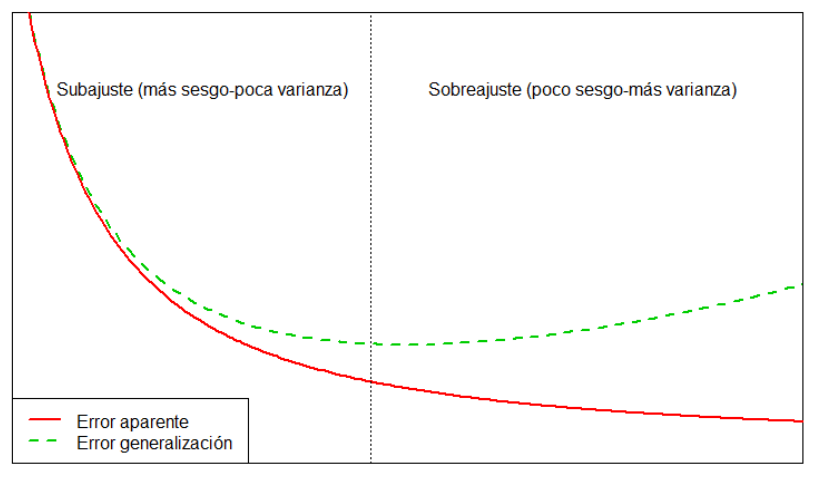
\includegraphics[width=\textwidth]{assets/overfitting_underfitting.png}
    \end{figure}
    \item \textbf{Validación cruzada:} Se pretende estimar el error esperado de generalización para comparar modelos.
    Se realiza una partición de la muestra patrón $\mathcal{Z}=\begin{pmatrix}\mathcal{Z}_1 \\ \mathcal{Z}_2\end{pmatrix}$ y se usarán solo las observaciones en $\mathcal{Z}_1$ para ajustar la regla y se comprobará con $\mathcal{Z}_2$. A continuación se exponen algunos métodos de \textbf{validación cruzada}
    \begin{itemize}
        \item \textbf{$K$-fold:} $K$ bloques de la muestra patrón. Se usan $K-1$ bloques para ajustar la regla y el otro para validarla. Se promedian los errores.
        \item \textbf{Leave-one-out:} Una observación no se usa para entrenar, se realiza lo mismo para todas las observaciones y se promedia el error.
        \item \textbf{Muestra aleatoria:} Se toma una muestra aleatoria como partición de la muestra patrón, se ajusta con ella y se usa el resto de observaciones para estimar el error (``.632Bootstrap'', ``out-of-bag''\dots).
    \end{itemize}
    \item \textbf{$m$-vecinos más proximos:} Sean $N_m(x)$ las $m$ observaciones más próximas a $x$. Se seguirá un método de votación en el cual se asigna a $K$ si
    \[
        \#\{x_i\in N_m(x)\enspace \text{con} \enspace g_i=K\}=\max_{1\leq k\leq q}\#\{x_i\in N_m(x)\enspace \text{con} \enspace g_i=k\}
    \]
    \newpage
    Problemas de sobreajuste cuando $m$ es muy pequeño o de subajuste cuando $m$ es demasiado grande.
    \begin{figure}[h]
        \centering
        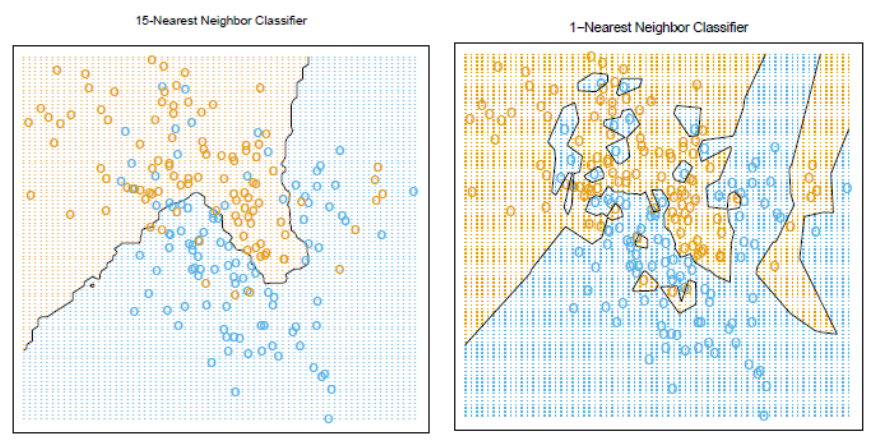
\includegraphics[width=\textwidth]{assets/k_neighbours.png}
    \end{figure}
    \item Árboles de clasificación: Son la base de métodos muy efectivos (Random Forest).
    \begin{figure}[h]
        \centering
        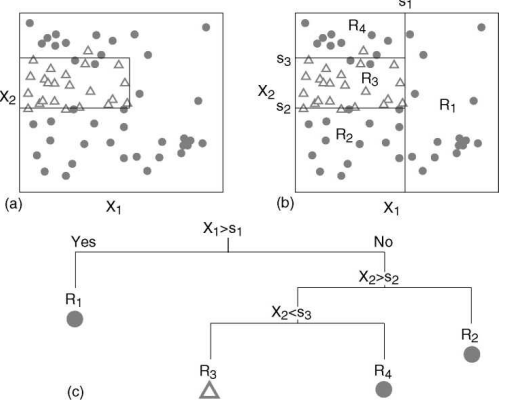
\includegraphics[width=0.8\textwidth]{assets/cart_classification.png}
    \end{figure}
    \newpage
    \item Suport Vector Machines (SVM): A partir de dos clases separables linealmente se busca el hiperplano que separa las clases con el mayor ``margen'' ($m$) posible.
    \begin{figure}[h]
        \centering
        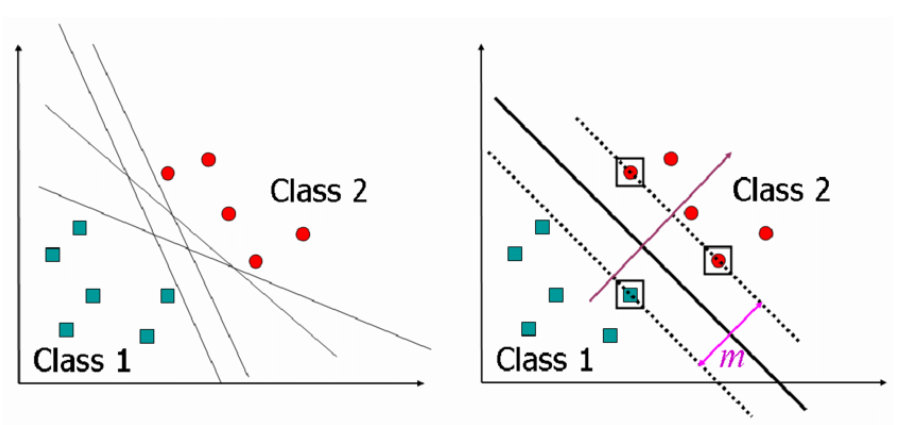
\includegraphics[width=\textwidth]{assets/svm_classification.png}
    \end{figure}
    
    En caso de que no sean separables se transforman los datos a un espacio de dimensión mayor donde si lo sean.
 \end{itemize}
